
\newpage
\section{\textbf{Mô hình,thực nghiệm và đánh giá}}

% \textbf{1. Hệ thống kiểm duyệt nội dung đa phương thức}


% \begin{figure}[H]
%     \centering
%     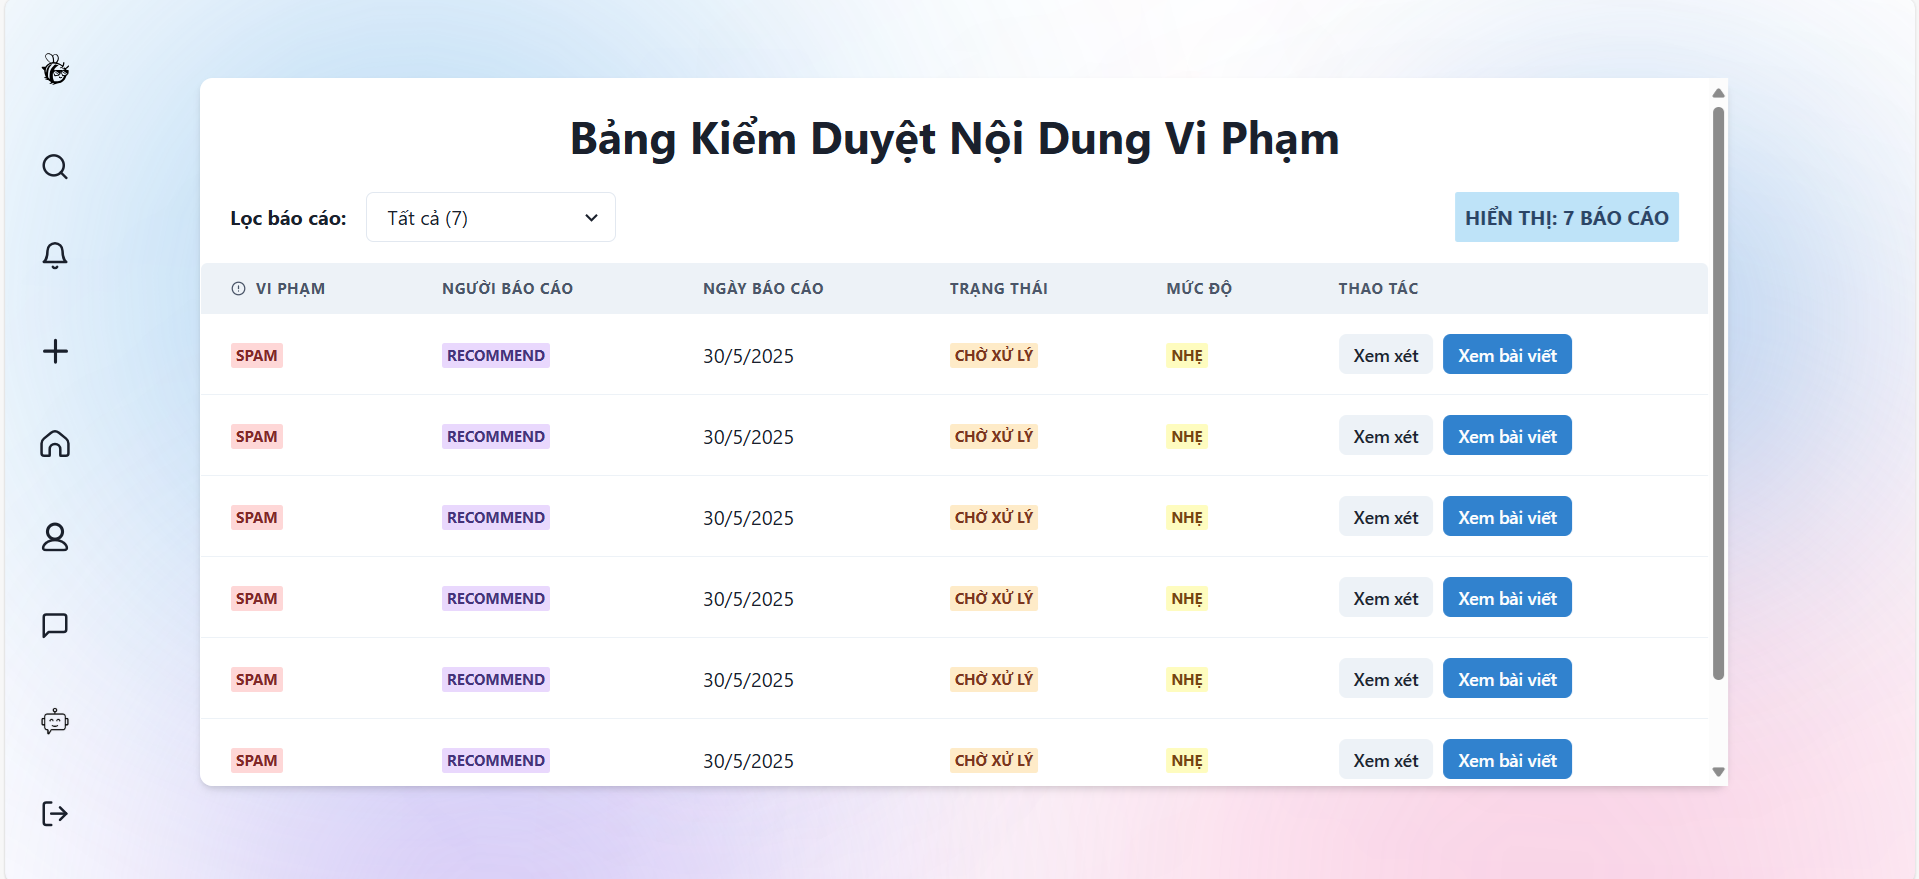
\includegraphics[width=1\textwidth]{image/thucnghiem/report.png}
%     \caption{Hình ảnh Bảng kiểm duyệt nội dung vi phạm}
%     \label{fig:bao_cao}
% \end{figure}



% \textbf{Phân tích thông minh với OpenAI Moderation API}
% \begin{itemize}
%     \item \textbf{Kiểm duyệt đa phương thức}: Phân tích cả văn bản và hình ảnh trong moderationService.ts
%     \item \textbf{Phân loại mức độ nghiêm trọng}: Tự động xác định low, medium, high dựa trên điểm số vi phạm
%     \item \textbf{Xử lý thời gian thực}: Kiểm tra ngay khi đăng bài, tạo báo cáo tự động trong moderationController.ts
% \end{itemize}

% \textbf{Dashboard quản trị viên}
% \begin{itemize}
%     \item Giao diện quản lý báo cáo vi phạm hoàn chỉnh trong AdminPage.tsx
%     \item Workflow phê duyệt/từ chối với lý do chi tiết
%     \item Thống kê vi phạm theo thời gian và mức độ
% \end{itemize}

% \newpage

% \textbf{2. Tìm kiếm ngữ nghĩa vector-based}

% \begin{figure}[H]
%     \centering
%     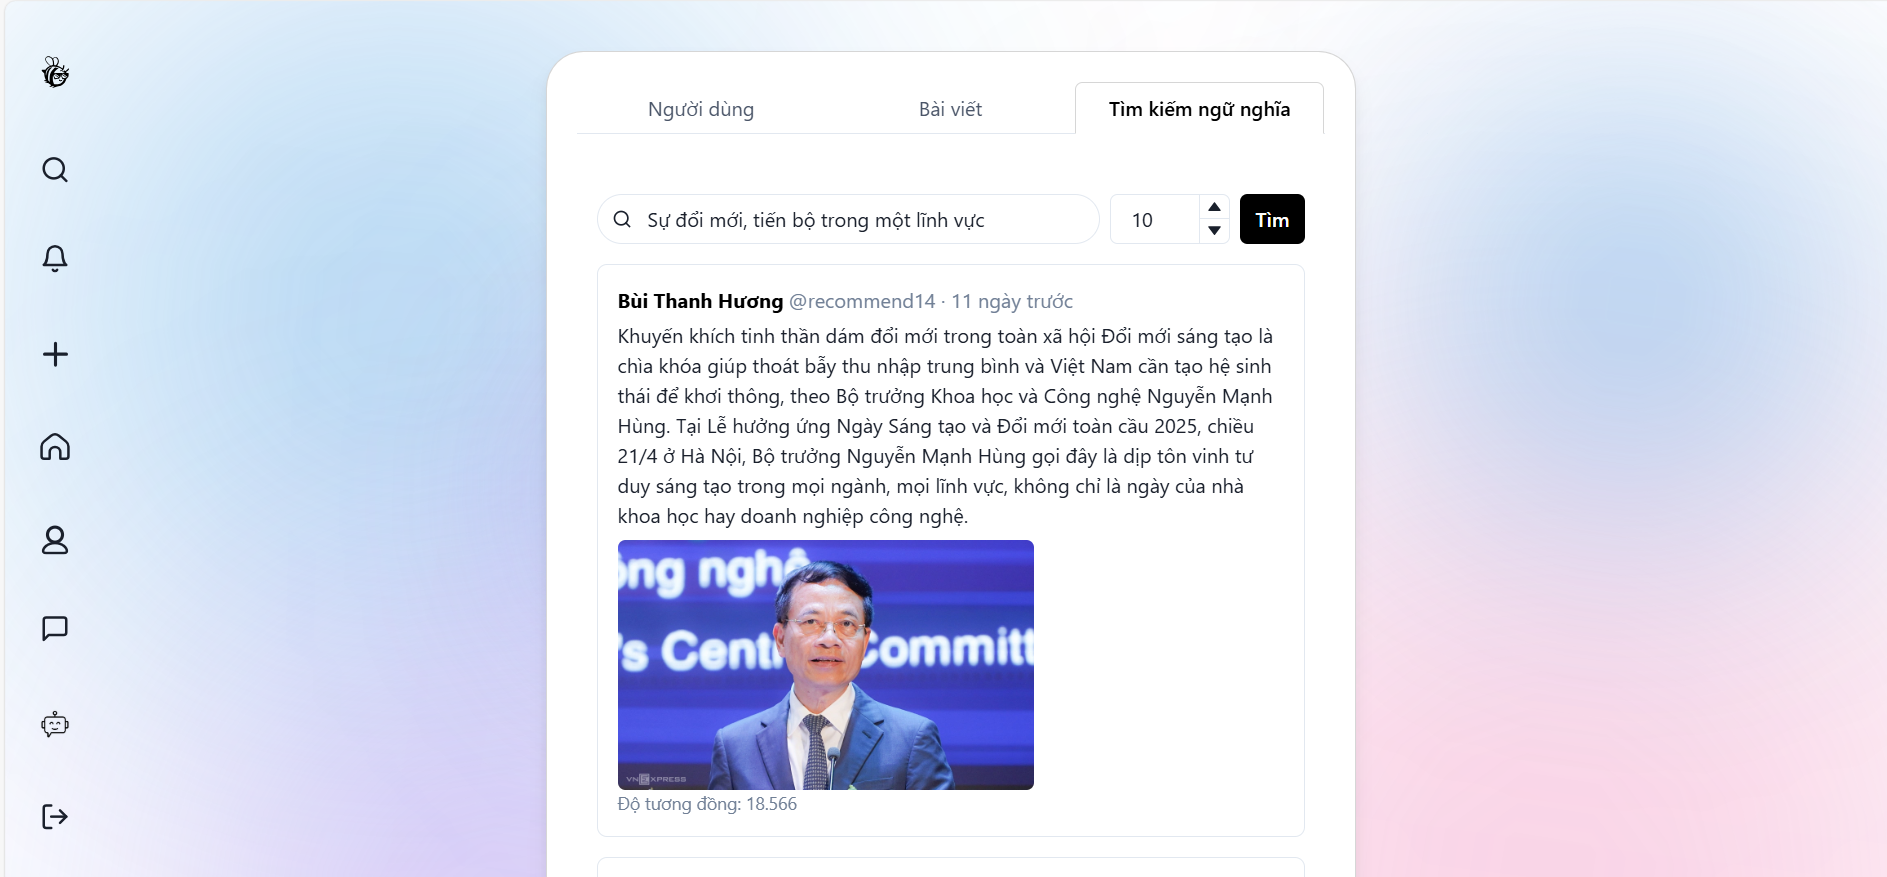
\includegraphics[width=1\textwidth]{image/thucnghiem/ngunghia.png}
%     \caption{Hình ảnh Ngữ nghĩa}
%     \label{fig:nghu_nghia}
% \end{figure}

% \begin{itemize}
%     \item \textbf{Vector embeddings}: Sử dụng OpenAI text-embedding-3-large trong embeddingService.ts
%     \item \textbf{Elasticsearch kNN}: Tìm kiếm vector với độ chính xác cao
%     \item \textbf{Tìm kiếm đa trường}: Kết hợp users, posts, comments trong một truy vấn
% \end{itemize}

% \textbf{Indexing thông minh}
% \begin{itemize}
%     \item \textbf{Auto-indexing}: Tự động tạo embeddings khi tạo bài viết mới
%     \item \textbf{Batch processing}: Script đánh index hàng loạt trong indexAdvancedData.ts
% \end{itemize}
% \newpage
% \textbf{3. Hệ thống nhắn tin thời gian thực}
% \begin{figure}[H]
%     \centering
%     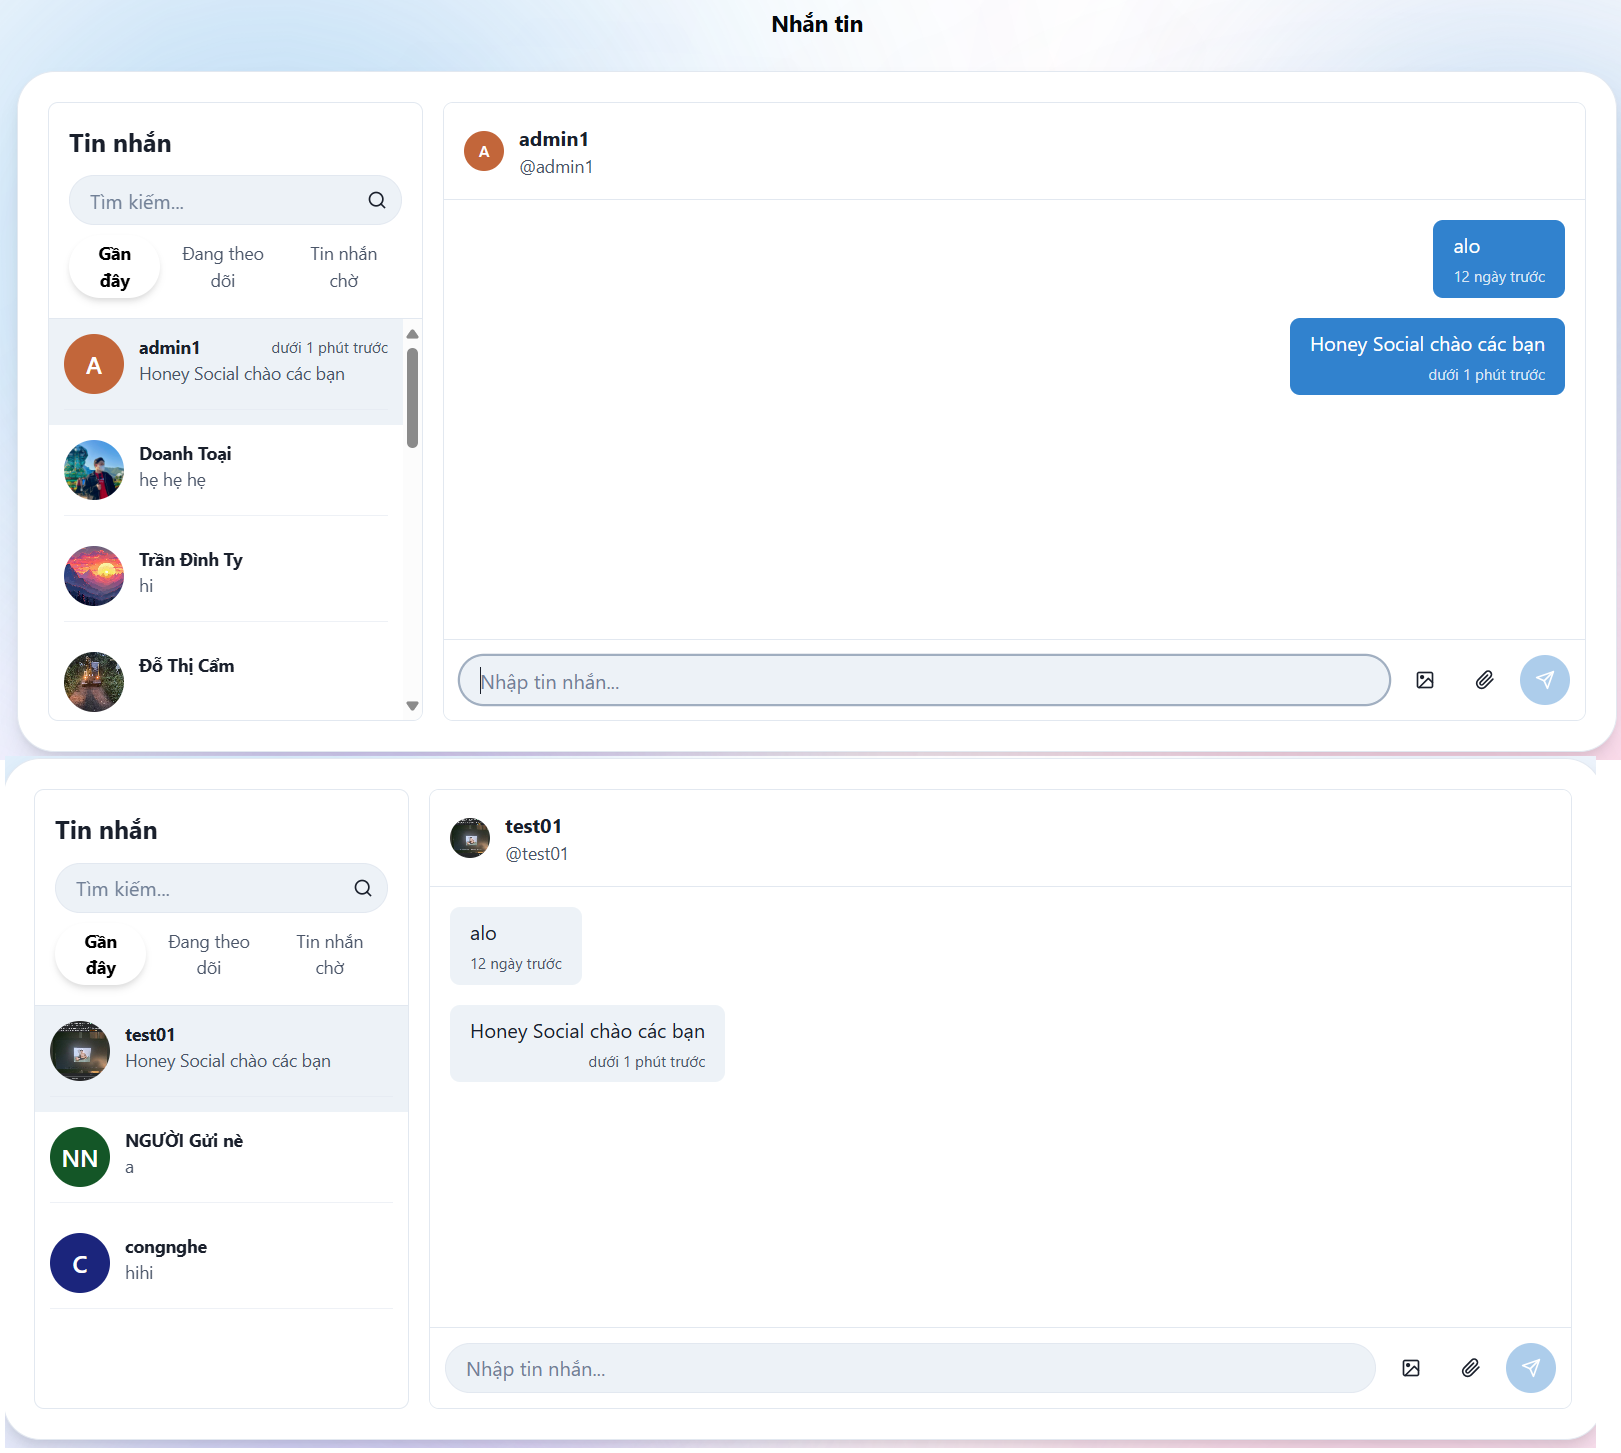
\includegraphics[width=1\textwidth]{image/thucnghiem/hinhve.png}
%     \caption{Hình ảnh Nhắn tin}
%     \label{fig:nhan_tin}
% \end{figure}
% \textbf{Tính năng nâng cao}
% \begin{itemize}
%     \item \textbf{Socket.io real-time}: Tin nhắn tức thời với read receipts trong socket.ts
%     \item \textbf{Message pending system}: Bảo vệ quyền riêng tư với workflow chấp nhận tin nhắn
%     \item \textbf{Media sharing}: Upload ảnh/file với Cloudinary integration
% \end{itemize}

% \textbf{Quản lý cuộc trò chuyện}
% \begin{itemize}
%     \item \textbf{Conversation management}: Giao diện chat với tabs Recent, Following, Pending
%     \item \textbf{Auto-follow on accept}: Tự động follow khi chấp nhận tin nhắn
%     \item \textbf{File upload}: Hỗ trợ nhiều định dạng với preview
% \end{itemize}

% \textbf{4. Hệ thống gợi ý thông minh}
% \begin{figure}[H]
%     \centering
%     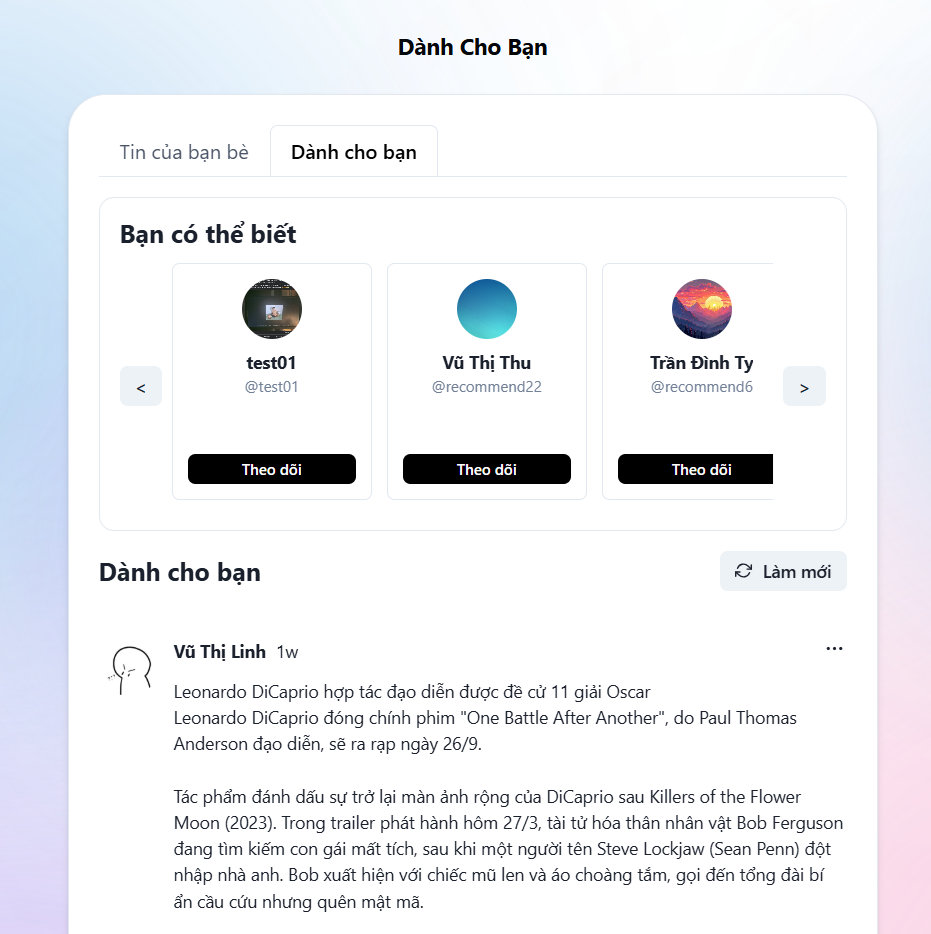
\includegraphics[width=1\textwidth]{image/thucnghiem/recommend.png}
%     \caption{Hình ảnh Gợi ý}
%     \label{fig:goi_y}
% \end{figure}
% \textbf{Gợi ý kết bạn dựa trên social graph}
% \begin{itemize}
%     \item \textbf{Mutual connections}: Phân tích kết nối chung trong recommendationController.ts
%     \item \textbf{Popularity scoring}: Tính điểm uy tín dựa trên followers/following ratio
%     \item \textbf{Elasticsearch aggregation}: Query phức tạp để tìm gợi ý tối ưu
% \end{itemize}

% \textbf{Gợi ý nội dung cá nhân hóa}
% \begin{itemize}
%     \item \textbf{Vector similarity}: So sánh embedding của bài viết đã thích
%     \item \textbf{Weighted combination}: Kết hợp nhiều vector với trọng số
%     \item \textbf{Fallback mechanism}: Đảm bảo luôn có gợi ý dù thiếu dữ liệu
% \end{itemize}

% \textbf{5. Trợ lý AI tích hợp}
% \begin{figure}[H]
%     \centering
%     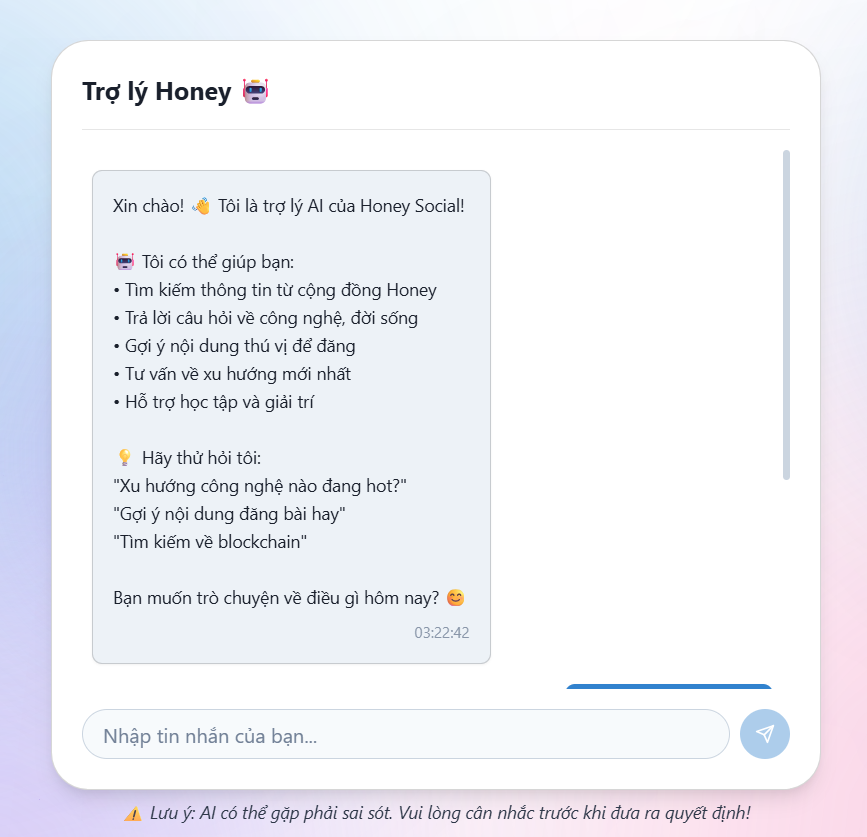
\includegraphics[width=1\textwidth]{image/thucnghiem/ai.png}
%     \caption{Hình ảnh Trí tuệ nhân tạo}
%     \label{fig:tri_tue_nhan_tao}
% \end{figure}
% \textbf{OpenAI Assistant với context}
% \begin{itemize}
%     \item \textbf{Thread-based conversation}: Lưu trữ lịch sử trò chuyện trong openaiService.ts
%     \item \textbf{Context awareness}: AI hiểu thông tin user như bio, posts, likes
%     \item \textbf{File search integration}: Tìm kiếm thông tin từ database
% \end{itemize}

% \textbf{Giao diện chat thông minh}
% \begin{itemize}
%     \item \textbf{Quick suggestions}: Gợi ý câu hỏi nhanh trong ChatAI.tsx
%     \item \textbf{Real-time typing}: Hiệu ứng typing indicator
%     \item \textbf{Message history}: Lưu trữ và khôi phục cuộc trò chuyện
% \end{itemize}

% \textbf{6. Hệ thống xác minh email}
% \begin{figure}[H]
%     \centering
%     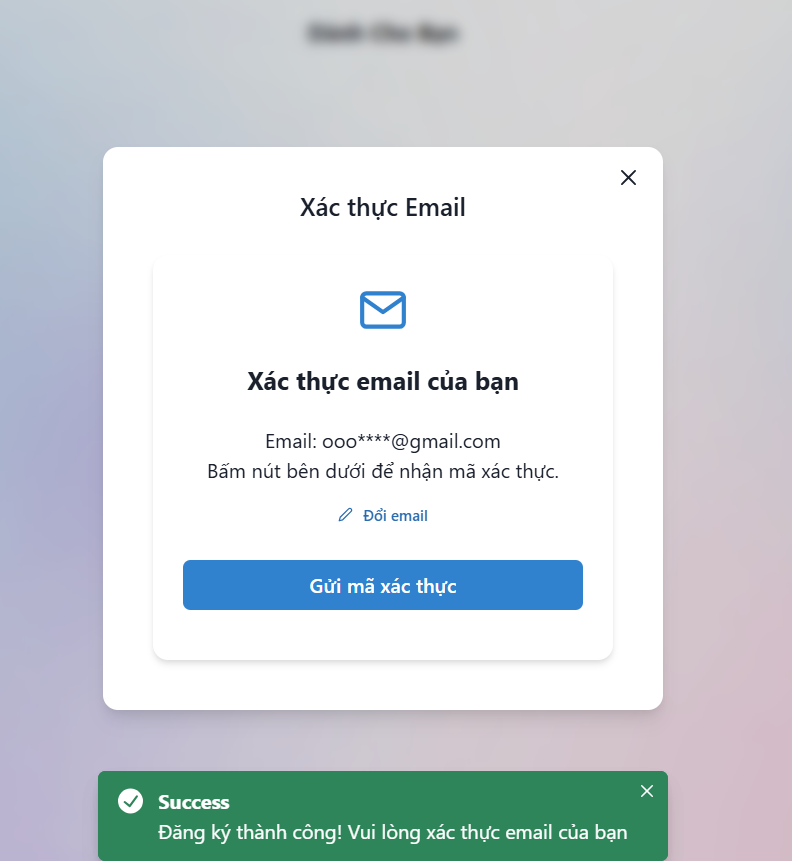
\includegraphics[width=1\textwidth]{image/thucnghiem/mail.png}
%     \caption{Hình ảnh Xác nhận mail}
%     \label{fig:xac_nhan}
% \end{figure}
% \textbf{Security với UX tối ưu}
% \begin{itemize}
%     \item \textbf{Rate limiting}: Chống spam với cooldown 45 giây trong verificationController.ts
%     \item \textbf{Email masking}: Bảo mật thông tin email
%     \item \textbf{Protected routes}: Component bảo vệ yêu cầu xác minh trong EmailProtectedRoute.tsx
% \end{itemize}

% \textbf{Workflow hoàn chỉnh}
% \begin{itemize}
%     \item \textbf{Email change flow}: Quy trình đổi email an toàn
%     \item \textbf{Queue processing}: Xử lý email bất đồng bộ
%     \item \textbf{Modal integration}: Giao diện xác minh liền mạch
% \end{itemize}

% \textbf{Background processing}
% \begin{itemize}
%     \item \textbf{Social actions worker}: Xử lý like/follow bất đồng bộ trong socialActionsWorker.ts
%     \item \textbf{Queue-based architecture}: Tách biệt logic nặng khỏi response time
%     \item \textbf{Error handling}: Retry mechanism và fallback
% \end{itemize}
% \newpage
% \textbf{7. Bảo mật và triển khai}
% \begin{figure}[H]
%     \centering
%     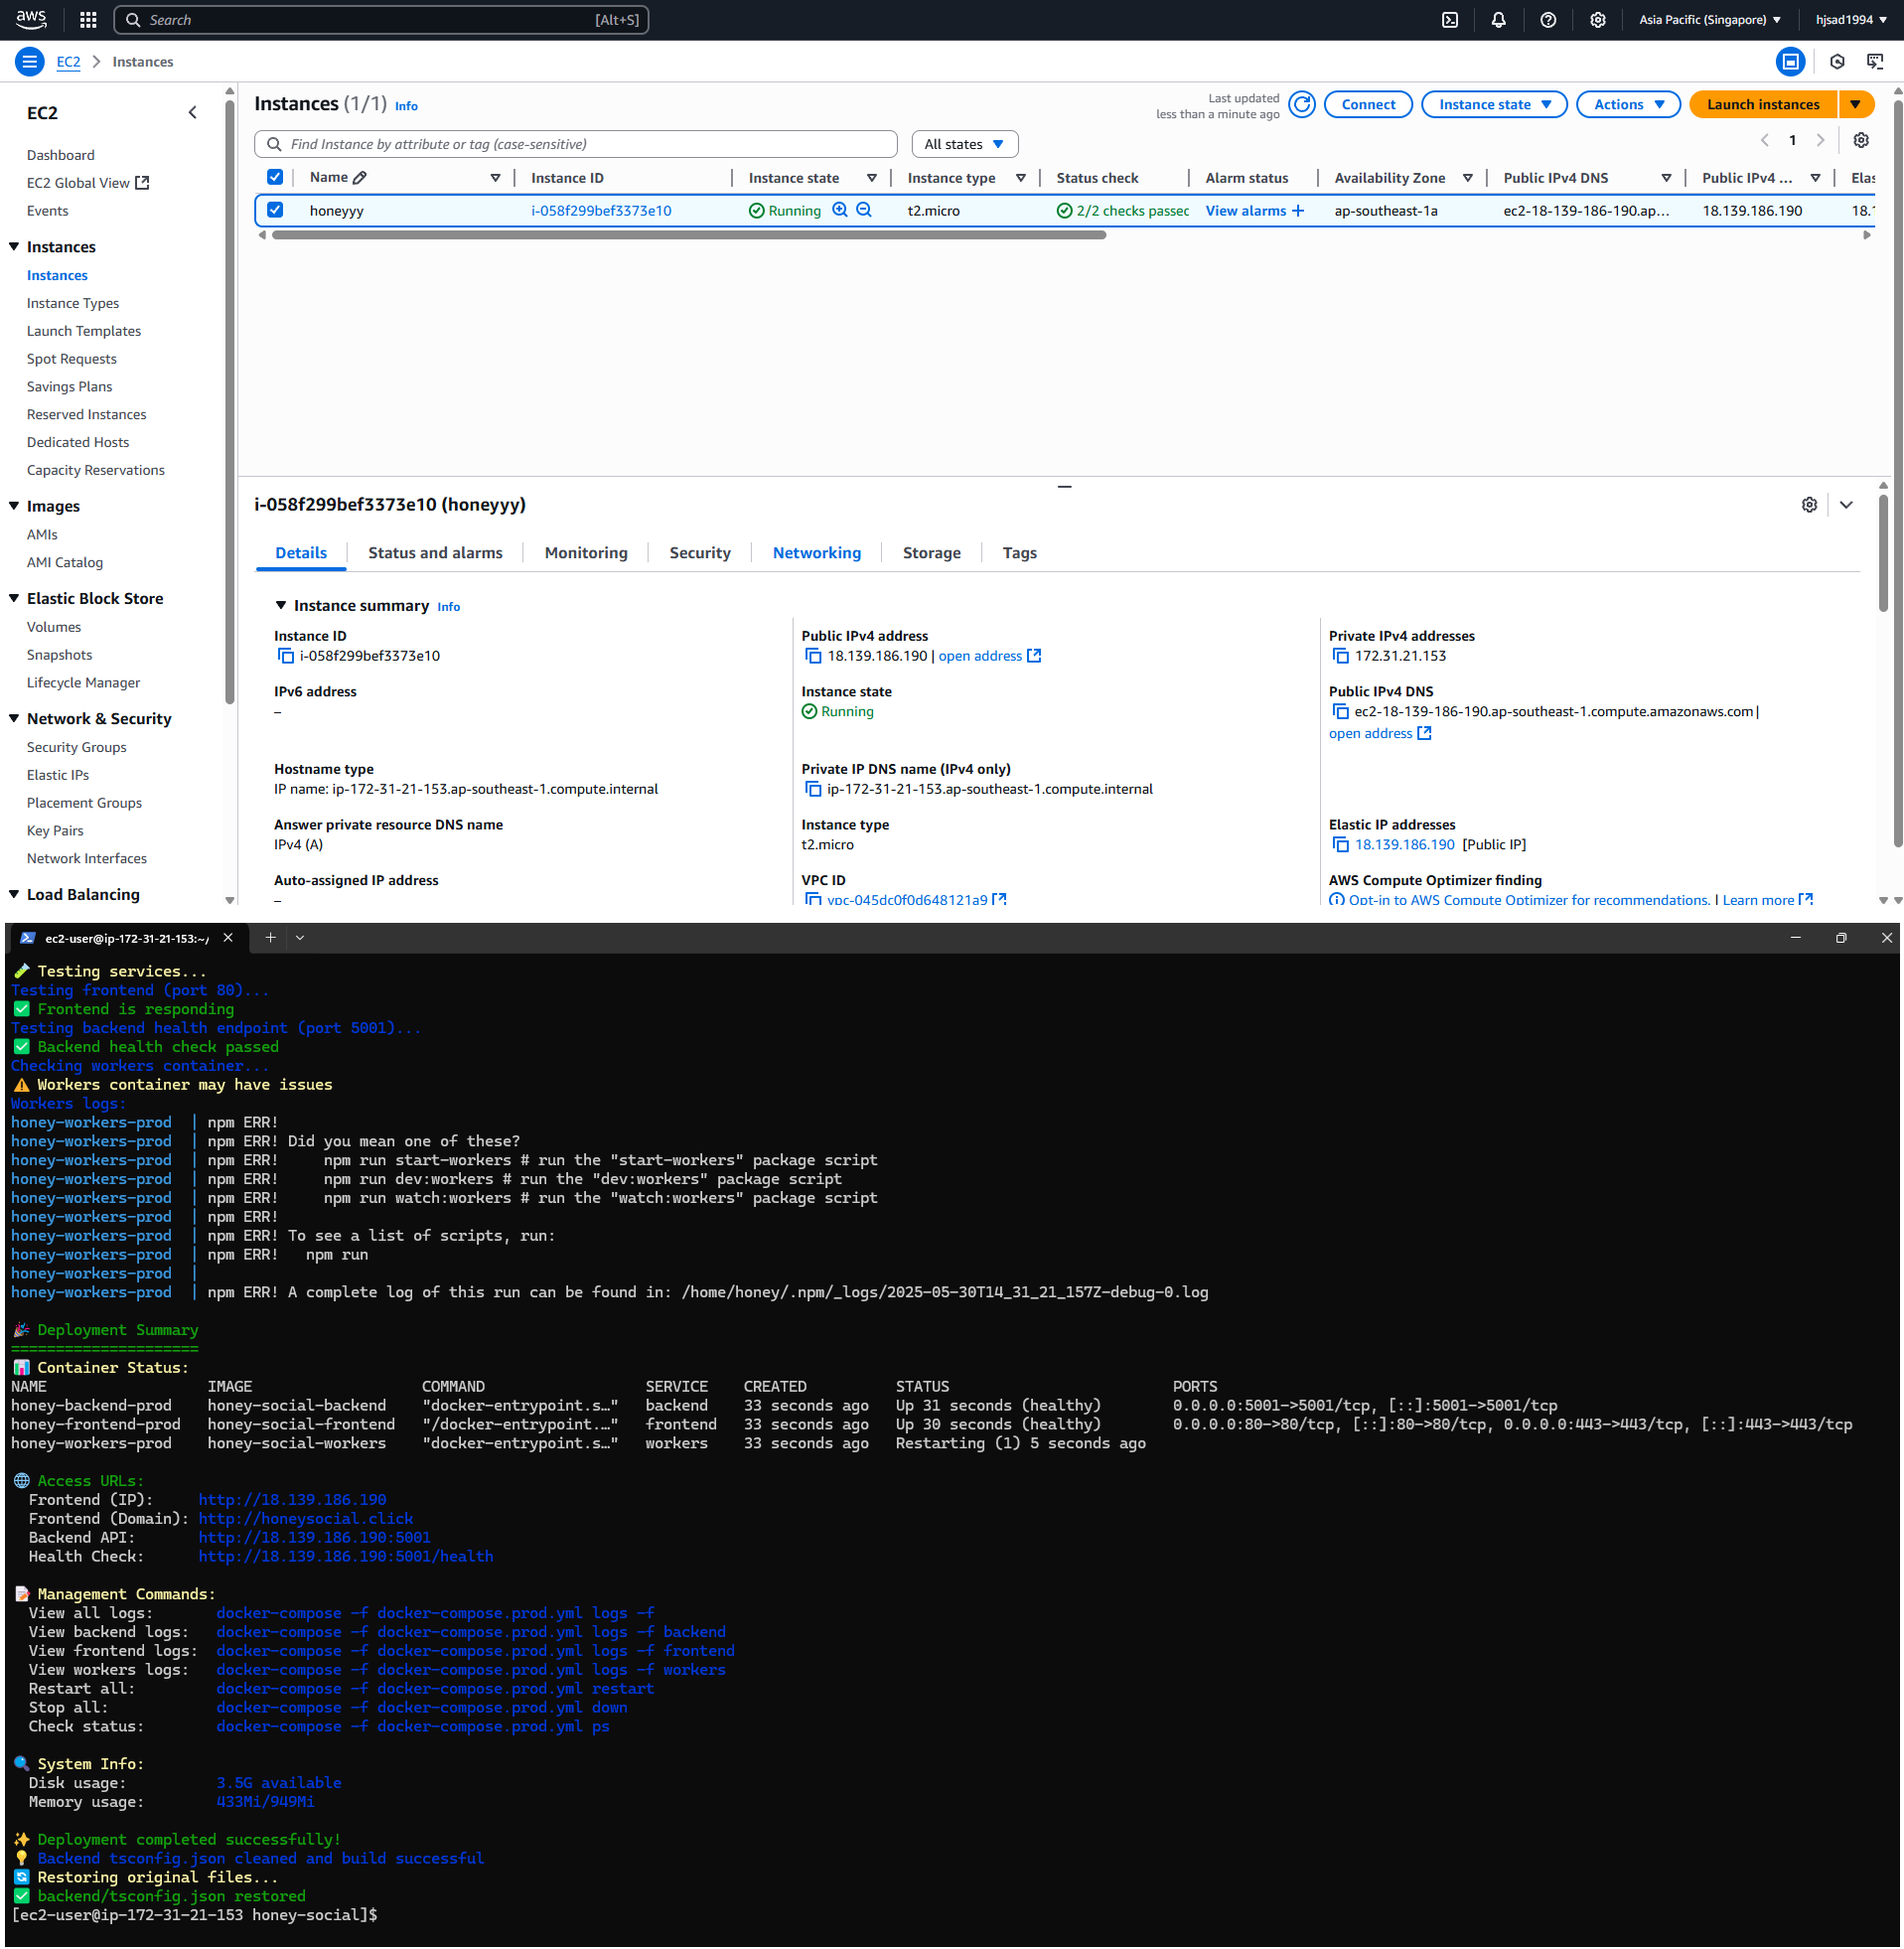
\includegraphics[width=1\textwidth]{image/thucnghiem/Deployment.png}
%     \caption{Hình ảnh Deployment}
%     \label{fig:deployment}
% \end{figure}

% \textbf{SSL Certificate tự động}
% \begin{itemize}
%     \item \textbf{Let's Encrypt SSL}: Certificate miễn phí cho domain honeysocial.click
%     \item \textbf{Auto-renewal}: Script tự động gia hạn certificate
%     \item \textbf{HTTPS redirect}: Tự động chuyển hướng từ HTTP sang HTTPS
% \end{itemize}

% \textbf{Deployment hoàn chỉnh}
% \begin{itemize}
%     \item \textbf{Docker containerization}: Triển khai với docker-compose
%     \item \textbf{Nginx reverse proxy}: Load balancing và SSL termination
%     \item \textbf{Production monitoring}: Health checks và logging
% \end{itemize}
